\begin{greek}
\chapter{Συλλογή σκουπιδιών με αντιγραφή}\label{ch:cop}
Η συλλογή με σήμανση και εκκαθάριση έχει σχετικά μικρό κόστος,
ωστόσο ενδέχεται η μνήμη να κατακερματίζεται. Η συλλογή σκουπιδιών
πρέπει να καταλαμβάνει τον ελάχιστο δυνατό χρόνο εκτέλεσης σε
ένα καλώς διαμορφωμένο σύστημα και καθώς το κόστος των εργασιών 
μνήμης του τροποποιητή κυριαρχεί έναντι αυτού του συλλέκτη η
εκχώρηση μνήμης πρέπει να είναι γρήγορη. Η συλλογή με σήμανση
και συμπύκνωση εξαλείφει τον κατακερματισμό της μνήμης και 
υποστηρίζει πολύ γρήγορη εκχώρηση μνήμης με τίμημα την αύξηση 
του χρόνου συλλογής αφού ο σωρός διατρέχεται πολλές φορές. Στο 
παρόν κεφάλαιο παρουσιάζεται η \textbf{συλλογή σκουπιδιών με 
αντιγραφή (copying garbage collection)}, η οποία ανακαλύφθηκε 
από τους Fenichel και Yochelson \cite{DBLP:journals/cacm/FenichelY69} 
και Cheney \cite{DBLP:journals/cacm/Cheney70}. Η συλλογή με 
αντιγραφή συμπυκνώνει το σωρό, επιτρέποντας γρήγορη εκχώρηση
μνήμης και επίσης πραγματοποιεί μόνο ένα πέρασμα στο σωρό. Το 
βασικό μειονέκτημα είναι πώς το μέγεθος της διαθέσιμης μνήμης 
στο σωρό μειώνεται στο μισό.

\section{Αντιγραφή μεταξύ ημιχώρων}
Η βασική εκδοχή ενός συλλέκτη αντιγραφής διαιρεί το σωρό σε δύο 
ισομεγέθεις \textbf{ημιχώρους}, το \textbf{χώρο-από} και το \textbf{χώρο-προς}.
Εάν υπάρχει διαθέσιμη μνήμη για ένα αντικείμενο, αυτή εκχωρείται στο χώρο-προς 
αυξάνοντας την τιμή ενός δείκτη $free$. Διαφορετικά, ο ρόλος των 
ημιχώρων εναλλάσσεται πριν ο συλλέκτης αντιγράψει όλα τα ζωντανά 
αντικείμενα από τον πρώην χώρο-προς (και νυν χώρο-από) στο νυν 
χώρο-προς (πρώην χώρο-από). Στο τέλος της συλλογής, όλα τα ζωντανά 
αντικείμενα είναι τοποθετημένα σε ένα πυκνό πρόθεμα του χώρου-προς. 
Ο συλλέκτης αγνοεί το χώρο-από και τα αντικείμενα που βρίσκονται σε 
αυτόν μέχρι την επόμενη συλλογή. Στην πράξη βέβαια, οι περισσότεροι 
συλλέκτες αντιγραφής μηδενίζουν το χώρο-από για ασφάλεια κατά την
αρχικοποίηση του επόμενου κύκλου συλλογής. 

Μετά την αρχικοποίηση, οι συλλέκτες αντιγραφής αντιγράφουν τα 
αντικείμενα ρίζες στο χώρο-προς. Τα αντικείμενα που έχουν αντιγραφεί 
αλλά όχι ακόμα εξεταστεί είναι γκρι. Κάθε πεδίο δείκτης ενός 
γκρι αντικειμένου περιέχει είτε την τιμή \textbf{null} είτε μία 
αναφορά προς ένα αντικείμενο του χώρου-από. Η διαδικασία \textproc{scan}
ενημερώνει κάθε πεδίο δείκτη ενός γκρι αντικειμένου, ο οποίος 
δείχνει σε κάποιο αντικείμενο του χώρου-από, με τη διεύθυνση 
του αντιγράφου του αντικειμένου στο χώρο-προς. 

\begin{algorithm}[H]
  \caption{Αντιγραφή: αρχικοποίηση και εκχώρηση}
  \label{alg:cop_1}
  \begin{algorithmic}[1]
    \Procedure{createSemispaces}{\null}
      \State $tospace \gets HeapStart$
      \State $extent \gets (HeapEnd-HeapStart)/2$ \Comment{size of a semispace}
      \State $top \gets fromspace$
      \State $free \gets tospace$
    \EndProcedure
    \Statex
    \Function{allocate}{$size$}
      \State \textbf{atomic}
      \State $result \gets free$
      \State $newfree \gets result + size$
      \If{$newFree > top$}
        \State \Return{\textbf{null}} \Comment{signal ``memory exhausted''}
      \EndIf
      \State $free \gets newfree$
      \State \Return{$result$}
    \EndFunction
  \end{algorithmic}
\end{algorithm}

Πιο συγκεκριμένα, 
για κάθε πεδίο δείκτη του ορίσματος της, καλεί τη διαδικασία 
\textproc{process}, η οποία με τη σειρά της, αν το όρισμα της 
δεν περιέχει την τιμή \textbf{null}, καλεί τη συνάρτηση \textproc{forward} 
με όρισμα το όρισμα με το οποίο αυτή κλήθηκε. Η συνάρτηση \textproc{forward} 
ελέγχει αν το αντικείμενο αναφοράς του ορίσματος της έχει ήδη 
αντιγραφεί στο χώρο-προς, και αν ναι, τότε επιστρέφει τη διεύθυνση 
του αντιγράφου. Αν όχι, καλεί τη συνάρτηση \textproc{copy} η 
οποία εκτελεί τις εξής ενέργειες: αποθηκεύει στη μεταβλητή $toRef$ 
την τιμή του δείκτη $free$, αυξάνει το δείκτη $free$ κατά το 
μέγεθος του αντικειμένου (όπως ακριβώς συμβαίνει και κατά την 
εκχώρηση μνήμης), μετακινεί (αντιγράφει) το αντικείμενο στη θέση 
$toRef$, αποθηκεύει στο πεδίο $forwardingAddress$ του αντικειμένου 
τη διεύθυνση του αντιγράφου του $toRef$ και τέλος, πριν επιστρέψει
τη μεταβλητή $toRef$, την προσθέτει στη λίστα εργασιών. Η αποθήκευση 
της διεύθυνσης ενός αντικειμένου στο πεδίο $forwardingAddress$ 
του αντιγράφου του στο χώρο-από από τη συνάρτηση \textproc{copy} 
εξασφαλίζει πώς η συλλογή με αντιγραφή διατηρεί την τοπολογία των 
ζωντανών αντικειμένων κατά την αντιγραφή τους από το χώρο-από στο
χώρο-προς. Σε αντίθεση με τους περισσότερους συλλέκτες με σήμανση 
και συμπύκνωση, ένας συλλέκτης με αντιγραφή δεν απαιτεί κανένα 
επιπλέον πεδίο στην επικεφαλίδα ενός αντικειμένου. Οποιοδήποτε 
πεδίο στο αντίγραφο ενός αντικειμένου του χώρου-προς στο χώρο-από 
μπορεί να αποθηκεύσει τη διεύθυνση του αντικειμένου στο χώρο-προς, 
καθώς το αντίγραφο αυτό δεν πρόκειται να χρησιμοποιηθεί ξανά 
μετά το πέρας της συλλογής. Το γεγονός αυτό καθιστά τη συλλογή 
με αντιγραφή κατάλληλη ακόμη και για αντικείμενα χωρίς επικεφαλίδα.

Όπως και οι περισσότερες τεχνικές συλλογής σκουπιδιών με εξιχνίαση, 
έτσι και η συλλογή με αντιγραφή διατηρεί μια λίστα εργασιών την 
οποία και επεξεργάζεται μέχρις ότου αυτή εκκενωθεί. Η λίστα εργασιών 
δύναται να υλοποιηθεί με διαφορετικούς τρόπους, οδηγώντας σε 
διαφορετική σειρά διάσχισης του γράφου αντικειμένων και διαφορετικές 
απαιτήσεις σε χώρο. Οι Fenichel και Yochelson \cite{DBLP:journals/cacm/FenichelY69}
υλοποιούν τη λίστα εργασιών ως μία απλή βοηθητική στοίβα, όπως 
κάνουν οι συλλέκτες με σήμανση και εκκαθάριση. Η αντιγραφή τελειώνει 
όταν η στοίβα είναι άδεια.

\begin{algorithm}[H]
  \caption{Αντιγραφή: αντιγραφή ημιχώρων}
  \label{alg:cop_2}
  \begin{algorithmic}[1]
    \Procedure{collect}{\null}
      \State \Call{flip}{\null}
      \State \Call{initialize}{$worklist$} \Comment{empty}
      \ForAll{$fld \; \textbf{in} \; Roots$} \Comment{copy the roots}
        \State \Call{process}{$fld$}
      \EndFor
      \While{\textbf{not} \Call{isEmpty}{$worklist$}} \Comment{copy transitive closure}
        \State $ref \gets$ \Call{remove}{$worklist$}
        \State \Call{scan}{$ref$}
      \EndWhile    
    \EndProcedure
    \Statex
    \Procedure{flip}{\null}
      \Comment{switch semispaces}
      \State $fromspace, tospace \gets tospace, \, fromspace$
       \State $top \gets tospace + extent$
      \State $free \gets tospace$
    \EndProcedure  
    \Statex
    \Procedure{scan}{$ref$}
      \ForAll{$fld \; \textbf{in} \; Pointers(Roots)$}
        \State \Call{process}{$fld$}      
      \EndFor
    \EndProcedure
    \Statex
    \Procedure{process}{$fld$} \Comment{update field with reference to tospace replica}
      \State $fromRef \gets *fld$
      \If{$fromRef \neq \textbf{null}$}
        \State $*fld \gets$ \Call{forward}{$fromRef$} \Comment{update with tospace reference}
      \EndIf
    \EndProcedure
    \Statex
    \Function{forward}{$fromRef$}
      \State $toRef \gets$ \Call{forwardingAddress}{$fromRef$}
      \If{$toRef = \textbf{null}$} \Comment{not copied (not marked)}
        \State $toRef \gets$ \Call{copy}{$fromRef$}
      \EndIf
      \State \Return{$toRef$}
    \EndFunction
    \Statex                                                  
    \Function{copy}{$fromRef$} \Comment{copy object and return forwarding address}
      \State $toRef \gets free$
      \State $free \gets free$ $+$ \Call{size}{$fromRef$}
      \State \Call{move}{$fromRef$, $toRef$}
      \State \Call{forwardingAddress}{$fromRef$} $\gets toRef$ \Comment{mark}
      \State \Call{add}{$worklist$, $toRef$}
      \State \Return{$toRef$}
    \EndFunction
  \end{algorithmic}
\end{algorithm}

Ο αλγόριθμος του Cheney \cite{DBLP:journals/cacm/Cheney70} χρησιμοποιεί
τα γκρι αντικείμενα του χώρου-προς ως μία ουρά. Η μόνη επιπλέον
μεταβλητή που χρησιμοποιεί είναι ο δείκτης $scan$, ο οποίος κάθε
χρονική στιγμή αναφέρεται στο επόμενο μη σαρωμένο αντικείμενο.
Όταν οι δύο ημιχώροι εναλλάσσονται οι δείκτες $scan$ και $free$
αρχικοποιούνται ώστε να δείχνουν στην αρχή του χώρου-προς (η
διαδικασία \textproc{initialize} εγγράφει το δείκτη $scan$ με
την τιμή του δείκτη $free$, ο οποίος στη διαδικασία \textproc{flip}
ενημερώθηκε με την διεύθυνση της αρχής του ημιχώρου-προς).
Αφού αντιγραφούν τα αντικείμενα ρίζες, η λίστα εργασιών, δηλαδή
το σύνολο των γκρι αντικειμένων αποτελείται ακριβώς από τα
αντιγεγραμμένα και όχι ακόμη σαρωμένα αντικείμενα στο χώρο-προς
μεταξύ των δεικτών $scan$ και $free$. Αυτή ακριβώς είναι και η
αναλλοίωτη που διατηρείται κατά τη διάρκεια της συλλογής. Ο
δείκτης $scan$ αυξάνεται καθώς πεδία αντικειμένων του χώρου-προς
σαρώνονται και ενημερώνονται. Η συλλογή ολοκληρώνεται όταν η
λίστα εργασιών είναι κενή: όταν ο δείκτης $scan$ συναντήσει το
δείκτη $free$. Η υλοποίηση είναι πολύ απλή: η συνάρτηση \textproc{isEmpty}
συγκρίνει τις τιμές των δεικτών $scan$ και $free$, η συνάρτηση
\textproc{remove} απλώς επιστρέφει την τιμή του δείκτη $scan$
και τέλος η διαδικασία \textproc{add} δεν προβαίνει σε καμία
ενέργεια.

\begin{algorithm}[H]
  \caption{Αντιγραφή: υλοποίηση λίστας εργασιών κατά Cheney}
  \label{alg:c_3}
  \begin{algorithmic}[1]
    \Procedure{initialize}{\null}
      \State $scan \gets free$
    \EndProcedure
    \Statex
    \Function{isEmpty}{$worklist$}
      \State \Return{$scan = free$}
    \EndFunction
    \Statex
    \Function{remove}{$worklist$}
      \State $ref \gets scan$
      \State $scan \gets scan$ $+$ \Call{size}{$scan$}
      \State \Return{$ref$}
    \EndFunction
    \Statex
    \Procedure{add}{$worklist$, $ref$}
      \State /* $nop$ */
    \EndProcedure
  \end{algorithmic}
\end{algorithm}

\section{Σειρά διάταξης και τοπικότητα}
Η τοπικότητα τόσο του τροποποιητή όσο και του συλλέκτη μπορεί
να έχει σημαντική επίδραση στην επίδοση ενός προγράμματος. Όπως
είδαμε στο προηγούμενο κεφάλαιο ο συλλέκτης μπορεί να βλάψει
την τοπικότητα του τροποποιητή και επομένως και την επίδοση 
του τελευταίου εάν μετακινεί αντικείμενα σε τυχαίες νέες θέσεις 
χωρίς να λαμβάνει υπόψη σχέσεις μεταξύ δεικτών ή την αρχική 
διάταξη των αντικειμένων \cite{DBLP:conf/oopsla/AbuaiadhOPS04}. 
Ωστόσο, απαιτείται ο συμβιβασμός ανάμεσα στα οφέλη που προκύπτουν 
από την τοπικότητα του τροποποιητή και τη συχνότητα κλήσης του 
συλλέκτη. Ας συγκρίνουμε για παράδειγμα τη συλλογή με σήμανση 
και εκκαθάριση και τη συλλογή με αντιγραφή. Η συλλογή με σήμανση 
και εκκαθάριση έχει στη διάθεσή της διπλάσιο χώρο στο σωρό από 
ότι η συλλογή με αντιγραφή και αν υποθέσουμε πώς οι υπόλοιπες 
παράμετροι είναι ίδιες καταλήγουμε πώς η χρήση της πρώτης τεχνικής 
θα πραγματοποιήσει μισό αριθμό συλλογών. Οι Blackburn κ.ά. \cite{DBLP:conf/icse/BlackburnCM04} διαπιστώνουν πώς πράγματι η
συλλογή με σήμανση και εκκαθάριση παρουσιάζει καλύτερες συνολικά
επιδόσεις από τη συλλογή με αντιγραφή όταν ο σωρός είναι σχεδόν
γεμάτος. Αντίθετα, oι Blackburn και McKinley \cite{DBLP:conf/oopsla/BlackburnM03} βρίσκουν πώς
σε μεγάλους σωρούς, τα οφέλη τοπικότητας που προκύπτουν από τη 
σειριακή εκχώρηση μνήμης υπερνικούν την αποδοτικότητα χώρου
της συλλογής με σήμανση και εκκαθάριση, έχοντας ως αποτέλεσμα
καλύτερους ρυθμούς αστοχιών σε όλα τα επίπεδα της κρυφής μνήμης.

Οι Blackburn κ.ά. \cite{DBLP:conf/icse/BlackburnCM04} αντιγράφουν τα αντικείμενα κατά βάθος.
Αντίθετα, ο Cheney διασχίζει το γράφο των αντικειμένων κατά πλάτος. 
Παρότι η διάσχιση υλοποιείται ως μία γραμμική (και συνεπώς προβλέψιμη) 
σάρωση της λίστας εργασιών των γκρι αντικειμένων του χώρου-προς,
η αντιγραφή αντικειμένων κατά πλάτος επιδρά δυσμενώς στην τοπικότητα
του τροποποιητή καθώς τείνει να ξεχωρίζει γονείς και παιδιά.

\begin{figure}[H]
  \centering
  \begin{subfigure}{1.0\textwidth}
    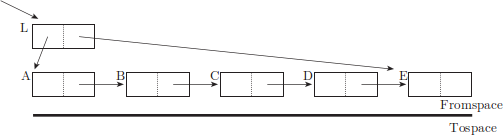
\includegraphics{figures/cop_1a}
    \caption{Ο χώρος-προς πριν τη συλλογή}
  \end{subfigure}

  \begin{subfigure}[b]{1.0\textwidth}
    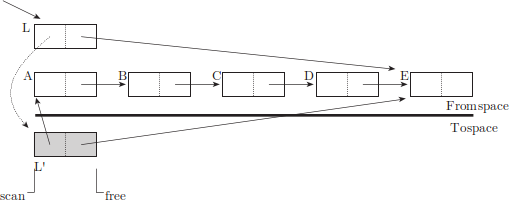
\includegraphics{figures/cop_1b}
    \caption{Αντιγραφή της ρίζας, L}
  \end{subfigure}
  
  \begin{subfigure}[b]{1.0\textwidth}
    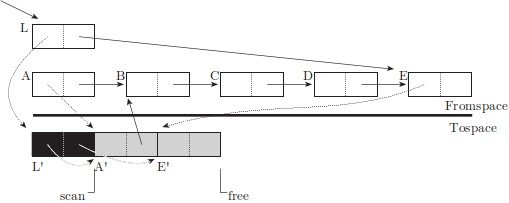
\includegraphics{figures/cop_1c}
    \caption{Σάρωση του αντιγράφου του L}
  \end{subfigure}
  \caption{Συλλογή με αντιγραφή: ένα παράδειγμα}
  \label{fig:cop_1}
\end{figure}

\begin{figure}[H]
  \ContinuedFloat
  \centering
  \begin{subfigure}{1.0\textwidth}
    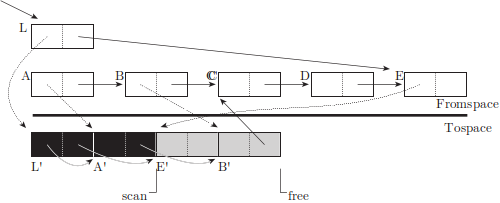
\includegraphics{figures/cop_2a}
    \caption{Σάρωση αντιγράφου του Α κ.ο.κ}
  \end{subfigure}

  \begin{subfigure}[b]{1.0\textwidth}
    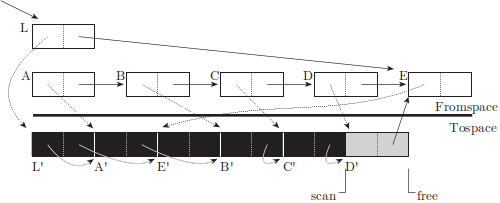
\includegraphics{figures/cop_2b}
    \caption{Σάρωση αντιγράφου του C}
  \end{subfigure}
  
  \begin{subfigure}[b]{1.0\textwidth}
    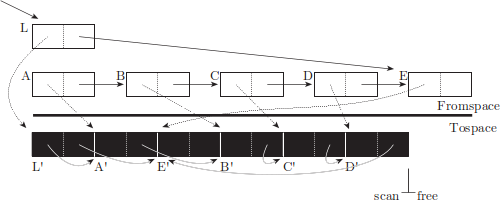
\includegraphics{figures/cop_2c}
    \caption{Σάρωση αντιγράφου του D. $scan=free$ και η 
             συλλογή ολοκληρώνεται.}
  \end{subfigure}
  \caption{Συλλογή με αντιγραφή: ένα παράδειγμα (συνέχεια)}
  \label{fig:cop_2}
\end{figure}

O White \cite{DBLP:conf/lfp/White80} ήταν ο πρώτος που συνέστησε τη χρήση του συλλέκτη
προς βελτίωση της επίδοσης του τροποποιητή. Τόσο η συλλογή με
αντιγραφή όσο και η συλλογή με σήμανση και συμπύκνωση μετακινούν
αντικείμενα, επηρεάζοντας με μεγάλη πιθανότητα την τοπικότητα
του τροποποιητή. Η ολισθαίνουσα μετακίνηση θεωρείται η βέλτιστη
όσον αφορά τη συλλογή με σήμανση και συμπύκνωση καθώς διατηρεί
τη διάταξη των αντικειμένων που έχει εγκαθιδρύσει ο εκχωρητής.
Η συντηρητική αυτή πολιτική είναι σίγουρα ασφαλής. Είναι όμως
και βέλτιστη; Η συλλογή με σήμανση και συμπύκνωση, η οποία 
συμπυκνώνει το σωρό επιτόπου είτε μετακινώντας ζωντανά αντικείμενα 
σε τρύπες είτε ολισθαίνοντας τα στο ένα άκρο του σωρού, δεν
έχει πολλές δυνατότητες τροποποίησης της διάταξης των αντικειμένων 
στο σωρό προς όφελος της τοπικότητας του τροποποιητή. Από την
άλλη πλευρά, οποιοσδήποτε αλγόριθμος συλλογής ο οποίος μετακινεί 
αντικείμενα σε μία φρέσκια περιοχή του σωρού χωρίς να καταστρέφει
τα αυθεντικά δεδομένα μπορεί να τα αναδιατάξει προκειμένου να
βελτιώσει την επίδοση του τροποποιητή.

Δυστυχώς υπάρχουν δύο λόγοι για τους οποίους δεν μπορούμε να
βρούμε μία βέλτιστη διάταξη των αντικειμένων που να ελαχιστοποιεί
τον αριθμό αστοχιών κρυφής μνήμης του προγράμματος. Πρώτον, ο
συλλέκτης δεν μπορεί να γνωρίζει το μοτίβο πρόσβασης των μελλοντικών
προσβάσεων σε αντικείμενα. Ακόμη χειρότερα, οι Petrank και Rawitz
\cite{DBLP:conf/popl/PetrankR02} αποδεικνύουν πώς το πρόβλημα της τοποθέτησης είναι NP-complete:
δεδομένης της τέλειας γνώσης των μελλοντικών προσβάσεων, δεν
υπάρχει αποδοτικός αλγόριθμος υπολογισμού μιας βέλτιστης τοποθέτησης.

\begin{algorithm}[H]
  \caption{Αντιγραφή: σχεδόν κατά-βάθος αντιγραφή (Moon)}
  \label{alg:c_4}
  \begin{algorithmic}[1]
    \Procedure{initialize}{$worklist$}
      \State $scan \gets free$
      \State $partialScan \gets free$
    \EndProcedure
    \Statex
    \Procedure{isEmpty}{$worklist$}
      \State \Return{$scan=free$} \Comment{as per Cheney}
    \EndProcedure
    \Statex
    \Procedure{remove}{$worklist$}
      \If{$partialScan < free$}
        \State $ref \gets partialScan$ \Comment{prefer secondary scan}
        \State $partialScan \gets partialScan$ $+$ \Call{size}{$partialScan$}
      \Else
        \State $ref \gets scan$ \Comment{primary scan}
        \State $scan \gets scan$ $+$ \Call{size}{$scan$}
      \EndIf
      \State \Return{$ref$}
    \EndProcedure
    \Statex
    \Procedure{add}{$worklist$, $ref$} \Comment{secondary scan on the most recently allocated page}
      \State $partialScan \gets$ \Call{max}{$partialScan$, $startOfPage(ref)$}
    \EndProcedure
  \end{algorithmic}
\end{algorithm}

Η μοναδική λύση στο πρόβλημα είναι η χρήση ευριστικών. Μια πιθανή
προσέγγιση είναι η χρήση της συμπεριφοράς του παρελθόντος για την
πρόβλεψη της συμπεριφοράς του μέλλοντος. Ορισμένοι ερευνητές 
χρησιμοποιούν είτε στατιστική ανάλυση (profiling) βασιζόμενοι στην υπόθεση
των Calder κ.ά. \cite{DBLP:conf/asplos/CalderKJA98} πώς τα προγράμματα συμπεριφέρονται παρόμοια
για διαφορετικές εισόδους, είτε online δειγματοληψία (online sampling)
βασιζόμενοι στην υπόθεση των Chilimbi κ.ά. \cite{DBLP:conf/pldi/ChilimbiHL99}
πώς η συμπεριφορά του προγράμματος παραμένει η ίδια από μία
περίοδο στην επόμενη. Μια άλλη ευριστική είναι η διατήρηση της
διάταξης εκχώρησης, όπως κάνει η ολισθαίνουσα συμπύκνωση. Μια
τρίτη στρατηγική αφορά την προσπάθεια τοποθέτησης παιδιών δίπλα
σε έναν από τους γονείς τους, αφού ο μόνος τρόπος πρόσβασης ενός
παιδιού είναι η φόρτωση μιας αναφοράς από κάποιον από τους γονείς
αυτού. Ο αλγόριθμος του Cheney υλοποιεί κατά πλάτος αντιγραφή
τείνοντας όμως να τοποθετεί κοντά μακρινά ξαδέρφια και όχι γονείς
με τα παιδιά τους.

Οι αρχικές μελέτες του πώς μπορεί να επωφεληθεί η τοπικότητα
του τροποποιητή από τη σειρά αντιγραφής των αντικειμένων επικεντρώνονται
στην ελαχιστοποίηση των σφαλμάτων σελίδας: ο απώτερος στόχος 
είναι η τοποθέτηση σχετιζόμενων αντικειμένων στην ίδια σελίδα.
Οι Stamos \cite{stamos1982large, DBLP:journals/tocs/Stamos84}
και Blau \cite{DBLP:journals/pe/Blau83} διαπιστώνουν μέσω προσομοιώσεων
πώς παρότι η κατά βάθος αντιγραφή είναι πιο επικερδής από την
κατά πλάτος αντιγραφή, αυτή οδηγεί σε χειρότερη συμπεριφορά όσον
αφορά τα σφάλματα σελίδων σε σχέση με την αρχική διάταξη δημιουργίας
των αντικειμένων. Ο Wilson κ.ά. \cite{DBLP:conf/pldi/WilsonLM91}
ωστόσο υποστηρίζουν πώς οι εν λόγω προσομοιώσεις δε λαμβάνουν
υπόψη τους την τοπολογία των πραγματικών προγραμμάτων των γλωσσών
Lisp και Smalltalk, τα οποία τείνουν να δημιουργούν δένδρα με
μεγάλο πλάτος και μικρό βάθος: οι δενδρικές δομές υλοποιούν
πίνακες κατακερματισμού και έχουν σχεδιασθεί με στόχο την καλύτερη
διασπορά των κλειδιών προς αποφυγή συγκρούσεων.

Ο αλγόριθμος των Fenichel και Yochelson υλοποιεί την κατά βάθος
διάσχιση με τη χρήση μιας βοηθητικής στοίβας. Είναι πάντως δυνατή
η επίτευξη μιας σχεδόν κατά πλάτος διάσχισης χωρίς τη χρήση
βοηθητικής στοίβας. Ο Moon \cite{DBLP:conf/lfp/Moon84} τροποποίησε
τον αλγόριθμο του Cheney για να πετύχει μία σχεδόν κατά βάθος
διάσχιση. Ο αλγόριθμος του Moon χρησιμοποιεί εκτός του αρχικού
δείκτη $scan$ έναν επιπλέον δείκτη, τον $partialScan$. Οποτεδήποτε
αντιγράφεται ένα αντικείμενο, ο αλγόριθμος του Moon εκκινεί μια
δευτερεύουσα σάρωση στην τελευταία σελίδα του χώρου-προς η οποία
δεν έχει ακόμη σαρωθεί πλήρως. Όταν αυτό συμβεί, η κύρια σάρωση
συνεχίζει από την πρώτη σελίδα που δεν έχει σαρωθεί πλήρως. Στην
πράξη, η λίστα εργασιών υλοποιείται ως ένα ζεύγος ουρών Cheney.
Αυτή η \textbf{ιεραρχική αποσύνθεση} πλεονεκτεί έναντι της κλασσικής
κατά βάθος εξερεύνησης όσον αφορά την τοποθέτηση γονέων και
παιδιών στην ίδια σελίδα.

Το μειονέκτημα του αλγορίθμου του Moon είναι πώς αντικείμενα
μπορεί να σαρώνονται δύο φορές, αφού αυτός καταγράφει μόνο ένα
ζεύγος δεικτών σάρωσης και κατά συνέπεια ξεχνά τα μπλοκ μεταξύ
των θέσεων $scan$ και $free$ που έχουν ήδη μερικώς σαρωθεί.
Πράγματι, όπως διαπίστωσαν o Wilson κ.ά. \cite{DBLP:conf/pldi/WilsonLM91}
το 30\% των αντικειμένων ενδέχεται να σαρωθεί εις διπλούν. Οι
τελευταίοι τροποποίησαν τον αλγόριθμο του Moon παρέχοντας σε
κάθε σελίδα τους δικούς της δείκτες $free$ και $scan$, με τη
λίστα εργασιών να περιλαμβάνει πλέον τα μπλοκ που έχουν σαρωθεί
μερικώς. Αυτό σημαίνει πώς η κύρια σάρωση δεν χρειάζεται να
επισκεφθεί ξανά αντικείμενα σελίδων που έχει ήδη επεξεργασθεί
η δευτερεύουσα σάρωση.

\begin{figure}[H]
  \centering
  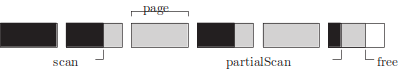
\includegraphics{figures/cop_4}
  \caption[Προσεγγιστική αντιγραφή κατά βάθος (Moon).]
   {Προσεγγιστική αντιγραφή κατά βάθος (Moon). Κάθε μπλοκ αναπαριστά
    μια σελίδα. Ως συνήθως, τα σαρωμένα πεδία είναι μαύρα, ενώ
    τα πεδία που έχουν αντιγραφεί αλλά όχι σαρωθεί ακόμη γκρι.
    Ο ελεύθερος χώρος απεικονίζεται με λευκό χρώμα.}
  \label{fig:cop_4}
\end{figure}

Η προσέγγιση του Moon είναι στατική και δε λαμβάνει υπόψη τη
συμπεριφορά των ξεχωριστών εφαρμογών. Είναι εμφανές ωστόσο πώς
τα οφέλη από την αναδιάταξη των αντικειμένων εξαρτώνται από τη
συμπεριφορά του τροποποιητή. Ο Lam κ.ά. \cite{DBLP:conf/iwmm/LamWM92}
διαπίστωσαν πώς ο αλγόριθμος του Moon παρουσιάζει ευαισθησία
όσον αφορά τη δομή και την ποικιλία των διαφόρων δομών δεδομένων
και εμφανίζει απογοητευτικές επιδόσεις για μη δενδροειδείς
δομές. Οι Siegwart και Hirzel \cite{DBLP:conf/iwmm/SiegwartH06}
επίσης παρατήρησαν πώς ένας παράλληλος συλλέκτης με ιεραρχική
αποσύνθεση ωφελεί σημαντικά την επίδοση μόνο ορισμένων benchmarks.

O Huang κ.ά. \cite{DBLP:conf/oopsla/HuangBMMWC04} παρακολουθούν
δυναμικά το προφίλ μιας εφαρμογής και προσπαθούν να αντιγράψουν
'θερμά' πεδία αντικειμένων δίπλα με τους γονείς αυτών. Αυτό το
σχήμα \textbf{online επαναδιάταξης αντικειμένων} καθώς και η
λειτουργία του φαίνονται στον αλγόριθμο~\ref{alg:cop_5} και το
σχήμα~\ref{fig:cop_3} αντίστοιχα. Ο βασικός βρόχος σάρωσης του
αλγορίθμου επεξεργάζεται πρώτα τη λίστα 'θερμών' αντικειμένων
και μετά τη λίστα ψυχρών αντικειμένων. Η υλοποίηση του μηχανισμού
δειγματοληψίας ως τμήμα ενός προσαρμοστικού δυναμικού μεταγλωττιστή
επιτρέπει τη φθηνή ταυτοποίηση των 'θερμών' αντικειμένων. Η υλοποίηση
των Huang κ.ά. επίσης λαμβάνει υπόψη τις αλλαγές της συμπεριφοράς
του τροποποιητή ανάμεσα στις διάφορες φάσεις λειτουργίας του,
επιτρέποντας στη 'θερμότητα' των πεδίων να φθίνει και να δειγματοληφθεί
ξανά. Τέλος, ο Huang κ.ά. διαπίστωσαν πώς η τεχνική της αντιγραφής
με online αναδιάταξη αντικειμένων εμφανίζει συγκρίσιμες ή και
καλύτερες επιδόσεις από στατικές τεχνικές όπως η αντιγραφή κατά
πλάτος.

\begin{algorithm}
  \caption{Αντιγραφή: online αναδιάταξη αντικειμένων}
  \label{alg:cop_5}
  \begin{algorithmic}[1]
    \Procedure{collect}{\null}
      \State \textbf{atomic}
      \State \Call{flip}{\null}
      \State \Call{initialize}{$hotList$, $coldList$}
      \ForAll{$fld \; \textbf{in} Roots$}
        \State \Call{adviceProcess}{$fld$}
      \EndFor
      \Repeat
        \While{\textbf{not} \Call{isEmpty}{$hotList$}}
          \State \Call{adviceScan}{$remove(hotList)$}
        \EndWhile
        \While{\textbf{not} \Call{isEmpty}{$coldList$}}
          \State \Call{adviceProcess}{$remove(coldList)$}
        \EndWhile
      \Until {\Call{isEmpty}{$hotList$}}
    \EndProcedure
    \Statex
    \Procedure{initialize}{$hotList$, $coldList$}
      \State $hotList \gets empty$
      \State $coldList \gets empty$
    \EndProcedure
    \Statex
    \Procedure{adviceProcess}{$fld$}
      \State $fromRef \gets *fld$
      \If{$fromRef \neq \textbf{null}$}
        \State $*fld \gets$ \Call{forward}{$fromRef$}
      \EndIf
    \EndProcedure
    \Statex
    \Procedure{adviceScan}{$obj$}
      \ForAll{$fld \; \textbf{in} Pointers(obj)$}
        \If{\Call{isHot}{$fld$}}
          \State \Call{adviceProcess}{$fld$}
        \Else
          \State \Call{add}{$coldList$, $fld$}
        \EndIf
      \EndFor
    \EndProcedure
  \end{algorithmic}
\end{algorithm}

\begin{figure}[H]
  \centering
  \begin{subfigure}{1.0\textwidth}
    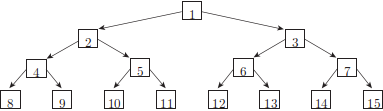
\includegraphics{figures/cop_3a}
    \caption{Το δένδρο προς αντιγραφή}
  \end{subfigure}

  \begin{subfigure}[b]{1.0\textwidth}
    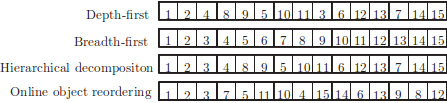
\includegraphics{figures/cop_3b}
    \caption{Τοποθέτηση αντικειμένων στο σωρό μετά την αντιγραφή}
  \end{subfigure}
  \caption[Αντιγραφή ενός δένδρου με διαφορετικές σειρές διάσχισης.]
    {Αντιγραφή ενός δένδρου με διαφορετικές σειρές διάσχισης.
     Κάθε γραμμή δείχνει πώς η αντίστοιχη σειρά διάσχισης τοποθετεί
     τα αντικείμενα στο χώρο-προς, υποθέτοντας πώς κάθε σελίδα
     χωράει τρία αντικείμενα.}
  \label{fig:cop_3}
\end{figure}

\section{Ανακεφαλαίωση και θέματα προς εξέταση}
\subsection{Εκχώρηση μνήμης}
Η εκχώρηση μνήμης σε έναν συμπυκνωμένο σωρό είναι γρήγορη επειδή
είναι απλή. Συνήθως απλώς απαιτεί τον έλεγχο έναντι ενός άνω 
ορίου (του σωρού ή ενός μπλοκ) και την υλοποίηση ενός δείκτη 
$free$. Εάν ο σωρός είναι οργανωμένος σε μπλοκ και όχι συνεχόμενος,
ο έλεγχος ενίοτε θα αποτυγχάνει στην οποία περίπτωση πρέπει να
δεσμευθεί ένα καινούριο μπλοκ. Η συχνότητα εμφάνισης της αργής
αυτής περίπτωσης θα εξαρτηθεί από το πώς μεταβάλλεται ο μέσος 
όρος μεγέθους των δημιουργούμενων αντικειμένων και το μέγεθος 
του μπλοκ. Η σειριακή εκχώρηση μνήμης επίσης είναι κατάλληλη
για χρήση σε πολυνηματικές εφαρμογές, καθώς σε κάθε νήμα τροποποιητή
μπορεί να δοθεί ένας τοπικός απομονωτής εκχώρησης χωρίς να
χρειάζεται ο συγχρονισμός με άλλα νήματα. Η οργάνωση αυτή είναι
απλή και απαιτεί τη χρήση μικρού αριθμού μεταδεδομένων, σε αντίθεση
με τοπικά σχήματα εκχώρησης για μη μετακινούντες συλλέκτες όπου
κάθε νήμα τροποποιητής μπορεί να χρειάζεται τις δικές του δομές
δεδομένων για την εκχώρηση μνήμης με ξεχωριστές ελεύθερες λίστες 
για αντικείμενα διαφορετικού μεγέθους.

Ο κώδικας που υλοποιεί τη σειριακή εκχώρηση είναι σύντομος 
και επιπλέον παρουσιάζει καλή συμπεριφορά όσον αφορά την κρυφή
μνήμη καθώς η εκχώρηση προχωράει σειριακά στο σωρό. Παρότι ο
συνδυασμός της σειριακής εκχώρησης, της μικρής διάρκειας ζωής
αντικειμένων και της οργάνωσης του σωρού σε ημιχώρους συνεπάγεται
πώς με μεγάλη πιθανότητα η επόμενη θέση μνήμης που θα εκχωρηθεί
είναι αυτή που έχει χρησιμοποιηθεί λιγότερο πρόσφατα, οι μηχανισμοί
προφόρτωσης των σύγχρονων επεξεργαστών συνήθως καλύπτουν την
λανθάνουσα καθυστέρηση που προκύπτει. Εάν όμως η συμπεριφορά
αυτή συγκρούεται με την πολιτική αντικατάστασης της λιγότερο 
πρόσφατα χρησιμοποιημένης σελίδας (LRU) του λειτουργικού
συστήματος σε βαθμό ώστε ο ρυθμός εναλλαγής σελίδων να χειροτερεύει
την επίδοση, τότε χρειάζεται επανεξέταση της διαμόρφωσης του
συστήματος διαχείρισης μνήμης. Η ικανοποιητική εκτέλεση της
εφαρμογής μπορεί να απαιτεί περισσότερη φυσική μνήμη ή αλλαγή
της πολιτικής συλλογής.

Ο Blackburn κ.ά. \cite{DBLP:conf/icse/BlackburnCM04} κατά την πειραματική μελέτη ενός
μικρού σχετικά benchmark διαπίστωσαν πώς παρότι η σειριακή
εκχώρηση υπερτερεί κατά 11\% έναντι της εκχώρησης με ελεύθερες
λίστες, η εκχώρηση καθεαυτή αποτελεί μόλις το 10\% του
συνολικού χρόνου εκτέλεσης μιας εφαρμογής. Επομένως η διαφορά
κόστους ανάμεσα στις δύο τεχνικές μπορεί να είναι αμελητέα.
Ωστόσο το κυρίαρχο κόστος της δημιουργίας ενός αντικειμένου 
συνήθως αφορά την αρχικοποίηση του αντικειμένου και όχι την
εκχώρηση μνήμης. Επιπλέον, τα αντικείμενα έχουν παρόμοιους
κύκλους ζωής σε πολλές εφαρμογές. Ο τροποποιητής δημιουργεί
έναν αριθμό από σημασιολογικά συνδεδεμένα αντικείμενα περίπου
την ίδια χρονική περίοδο, τα επεξεργάζεται και τα εγκαταλείπει
μαζικώς. Σε τέτοιες εφαρμογές η χρήση συμπυκνωμένου σωρού
προσφέρει υψηλή τοπική χωρικότητα αφού τα σχετιζόμενα αντικείμενα
τοποθετούνται στην ίδια σελίδα ή ακόμη και στο ίδιο μπλοκ
κρυφής μνήμης αν είναι μικρά. Μια τέτοια διάταξη τείνει
εμφανώς να οδηγήσει σε χαμηλότερο ρυθμό αστοχιών κρυφής
μνήμης σε σύγκριση με την περίπτωση όπου η μνήμη των συσχετιζόμενων
αντικειμένων εκχωρείται μέσω ξεχωριστών ελεύθερων λιστών.

\subsection{Χώρος και τοπικότητα}
Το άμεσο μειονέκτημα της συλλογής με αντιγραφή ημιχώρων είναι
η ανάγκη διατήρησης ενός δεύτερου ημιχώρου, ο οποίος μερικές
φορές καλείται και \textbf{εφεδρικό αντίγραφο (copy reserve)}.
Δεδομένου ενός προϋπολογισμού μνήμης και αγνοώντας τις δομές
δεδομένων που είναι απαραίτητες για τη λειτουργία του συλλέκτη
η συλλογή με αντιγραφή προσφέρει μόνο το μισό χώρο του σωρού
σε σχέση με άλλες τεχνικές συλλογής σκουπιδιών. Το αποτέλεσμα
είναι πώς οι συλλέκτες με αντιγραφή θα πραγματοποιήσουν περισσότερους
κύκλους συλλογής από ότι άλλοι συλλέκτες. Εάν αυτό θα οδηγήσει
σε καλύτερη ή χειρότερη επίδοση εξαρτάται από τους διάφορους
συμβιβασμούς μεταξύ συλλέκτη και τροποποιητή, τα χαρακτηριστικά
της εφαρμογής και το ποσό της διαθέσιμης μνήμης σωρού.

Η απλή ασυμπτωτική ανάλυση πολυπλοκότητας μπορεί να προτιμήσει
τη συλλογή με αντιγραφή έναντι της συλλογής με σήμανση και
εκκαθάριση. Έστω $M$ το συνολικό μέγεθος του σωρού και $L$ το
συνολικό μέγεθος των ζωντανών αντικειμένων. Η συλλογή με αντιγραφή
πρέπει να αντιγράψει και σαρώσει τα ζωντανά αντικείμενα καθώς
και να ενημερώσει τους δείκτες αυτών. Η συλλογή με σήμανση και
εκκαθάριση από την άλλη πλευρά πρέπει να ανακαλύψει όλα τα ζωντανά
αντικείμενα και στη συνέχεια να εκκαθαρίσει όλο το σωρό.
Ο Jones \cite{DBLP:books/wi/JonesL96} ορίζει τη χρονική πολυπλοκότητα για τη συλλογή
με αντιγραφή και για τη συλλογή με σήμανση και εκκαθάριση ως:

\begin{align}
t_{copy} &= cL \\
 t_{MS} &= mL+sM
\end{align}

Το ποσό της μνήμης που ανακτάται από κάθε συλλογή είναι αντίστοιχα:

\begin{align}
m_{copy} &= \frac{M}{2}-L \\
 m_{MS} &= M-L
\end{align}

Έστω τώρα $r=\frac{L}{M}$ το ποσοστό της ζωντανής μνήμης, το
οποίο υποθέτουμε πώς είναι σταθερό. Η αποδοτικότητα ενός αλγορίθμου
μπορεί να περιγραφεί από το λόγο mark/cons, $e$, ο οποίος αντιπροσωπεύει
την εργασία του συλλέκτη ανά μονάδα ανακτημένης μνήμης.

\begin{align}
e_{copy} &= \frac{2cr}{1-2r} \\
 e_{MS} &= \frac{mr+s}{1-r}
\end{align}

\begin{figure}[H]
  \centering
  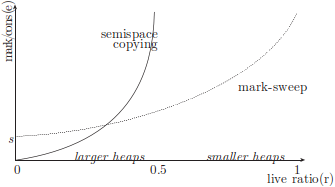
\includegraphics{figures/cop_5}
  \caption[Ρυθμοί mark/cons για συλλογή με σήμανση και εκκαθάριση
           και συλλογή με αντιγραφή.]
    {Ρυθμοί mark/cons για συλλογή με σήμανση και εκκαθάριση και
     συλλογή με αντιγραφή.}
  \label{fig:cop_5}
\end{figure}

Η συλλογή με αντιγραφή μπορεί να είναι πιο αποδοτική από τη
συλλογή με σήμανση και εκκαθάριση αν ο σωρός είναι αρκετά μεγάλος
και το $r$ αρκετά μικρό. Αυτή η απλουστευμένη ανάλυση ωστόσο
αγνοεί διάφορα ζητήματα. Οι σύγχρονοι συλλέκτες με σήμανση
και εκκαθάριση συνήθως χρησιμοποιούν οκνηρή εκκαθάριση, κάτι
που μειώνει τη σταθερά $s$ και κατ' επέκταση το λόγο $e_{MS}$.
Η ανάλυση της πολυπλοκότητας πρέπει να αντιμετωπισθεί με μεγάλη
προσοχή καθώς συνήθως αγνοεί λεπτομέρειες υλοποίησης παρότι
οι Hertz και Berger \cite{DBLP:conf/oopsla/HertzB05} επιβεβαιώνουν πειραματικά τη μορφή 
των καμπυλών (όπως ότι το κόστος της συλλογής με σήμανση και
εκκαθάριση είναι αντιστρόφως ανάλογο προς το μέγεθος του σωρού).
Οι πραγματικές λεπτομέρειες υλοποίησης παρότι είναι σημαντικές 
για πραγματικούς συλλέκτες δεν λαμβάνονται υπόψη από αναλύσεις
πολυπλοκότητας. Παράδειγμα μιας τέτοιας λεπτομέρειας αποτελεί
η θετική επίδραση στην τοπικότητα του τροποποιητή της χρήσης
σειριακής εκχώρησης μνήμης \cite{DBLP:conf/icse/BlackburnCM04}.

Επομένως η διαδοχική εκχώρηση μνήμης τείνει να τοποθετεί αντικείμενα
που προσπελάζονται ταυτόχρονα σε διαδοχικές θέσεις μνήμης, κάτι
που συμβάλλει στη βελτίωση του ρυθμού αστοχιών κρυφής μνήμης
του τροποποιητή. Ωστόσο η συλλογή με αντιγραφή αναδιατάσσει
τα επιζώντα αντικείμενα στο σωρό. Παρότι η συλλογή με αντιγραφή
κατά Cheney δεν χρειάζεται βοηθητική στοίβα για την καθοδήγηση
της εξιχνίασης, η διάσχιση κατά πλάτος τείνει να διαχωρίζει τους
γονείς από τα παιδιά τους. Η ιεραρχική αποσύνθεση προσφέρει
έναν καλό συμβιβασμό μεταξύ της πληρωμής του κόστους της βοηθητικής 
στοίβας και της βελτίωσης της διάταξης των αντικειμένων στο σωρό.
Ωστόσο παρότι η προσεκτική αναδιάταξη των αντικειμένων μπορεί
να είναι ωφέλιμη για μερικά προγράμματα, σε ορισμένες περιπτώσεις
η επίδρασή της μπορεί να αποδειχθεί αμελητέα. Τα περισσότερα
αντικείμενα έχουν μικρή διάρκεια ζωής και δεν επιβιώνουν ούτε
μία συλλογή. Επιπλέον, όπως παρατηρούν οι Blackburn και McKinley
\cite{DBLP:conf/oopsla/BlackburnM03}, πολλές εφαρμογές εστιάζουν τις προσβάσεις στη μνήμη και
ιδιαίτερα τις εγγραφές σε αυτά τα νέα αντικείμενα. Η πολιτική
διάσχισης ενός συλλέκτη δεν μπορεί προφανώς να επηρεάσει την
ιδιότητες τοπικότητας αντικειμένων που δεν μετακινούνται.

\subsection{Μετακίνηση αντικειμένων}
Η επιλογή ενός συλλέκτη αντιγραφής εξαρτάται μεταξύ άλλων από το
αν επιτρέπεται η μετακίνηση αντικειμένων καθώς από το κόστος της
μετακίνησης. Σε μερικά περιβάλλοντα δεν επιτρέπεται η μετακίνηση
αντικειμένων. Ένας από τους λόγους είναι η έλλειψη πληροφορίας
τύπων που καθιστά μη ασφαλή την τροποποίηση ενός πεδίου που είναι
πιθανόν δείκτης σε ένα αντικείμενο. Ένας διαφορετικός λόγος είναι
πώς μπορεί μια αναφορά προς ένα αντικείμενο να έχει μεταβιβασθεί 
ως σε μη διαχειρίσιμο κώδικα (για παράδειγμα ως όρισμα σε κάποια
κλήση συστήματος). Επιπλέον το πρόβλημα της εύρεσης δεικτών πολύ
συχνά είναι απλούστερο συλλογή με σήμανση και εκκαθάριση από ότι
στη συλλογή με αντιγραφή. Αρκεί η ανακάλυψη τουλάχιστον μιας
αναφοράς προς ένα ζωντανό αντικείμενο όταν χρησιμοποιείται ένας
μη μετακινών συλλέκτης. Από την άλλη πλευρά, ένας μετακινών
συλλέκτης πρέπει να εντοπίσει και ενημερώσει όλες τις αναφορές
προς ένα μετακινηθέν αντικείμενο. Όπως θα δούμε και στο κεφάλαιο
\ref{ch:concurrent}, το γεγονός αυτό καθιστά την ταυτόχρονη συλλογή
με μετακίνηση σημαντικά δυσκολότερη από την ταυτόχρονη συλλογή 
χωρίς μετακίνηση καθώς όλες οι ενημερώσεις των αναφορών προς
κάθε αντικείμενο πρέπει να εμφανίζονται ως ατομικές.

Η αντιγραφή ορισμένων αντικειμένων είναι ακριβή. Παρότι η
αντιγραφή ενός μικρού αντικειμένου κοστίζει περισσότερο από
τη σήμανση αυτού, το κόστος και η λανθάνουσα καθυστέρηση της
αντιγραφής συχνά κρύβονται από το κόστος της παρακολούθησης
δεικτών και της ανακάλυψης πληροφορίας τύπων. Από την άλλη
πλευρά η επαναλαμβανόμενη αντιγραφή μεγάλων αντικειμένων μπορεί
να οδηγήσει σε φτωχές επιδόσεις. Μια λύση είναι η αποφυγή
της αντιγραφής τους και η ανάθεση της διαχείρισής τους σε
έναν μη μετακινούντα συλλέκτη. Μια άλλη λύση είναι η αντιγραφή
τους να πραγματοποιείται εικονικά και όχι φυσικά.

\end{greek}
